\documentclass[a4paper,conference]{IEEEtran}
\usepackage{cleveref}
% *** GRAPHICS RELATED PACKAGES ***
\usepackage[pdftex]{graphicx}
\DeclareGraphicsExtensions{.pdf,.jpeg,.png,.svg}
\usepackage{svg}
\usepackage{tabularx}
% correct bad hyphenation here
\hyphenation{op-tical net-works semi-conduc-tor}
\bibliographystyle{IEEEtran}

% =============== DOCUMENT ===============
\begin{document}

% =============== TITLE ===============
% \title{Comparison of TLS 1.2 to TLS 1.3 and QUIC}
\title{New Features in TLS 1.3 and\\ TLS Integration into QUIC}

% =============== AUTHORS ===============
\author{\IEEEauthorblockN{Dorian Hanjo Loeben}
\IEEEauthorblockA{RWTH Aachen University\\
dorian.loeben@rwth-aachen.de}
\and
\IEEEauthorblockN{Nikita Malyschkin}
\IEEEauthorblockA{RWTH Aachen University\\
nikita.malyschkin@rwth-aachen.de}}



\maketitle

% =============== ABSTRACT ===============
\begin{abstract}
Recently the new Transport Layer Protocol 1.3 specifications got finalized and a few key features got changed.
In this paper we will be looking at the changes TLS 1.3 brought us. First we will focus on changes made in comparison to the TLS 1.2 standard.
After a general introduction to the changes we will have a closer look at the new 0-RTT handshake, its advantages and potential risks it brings.
At the end we will compare the new TLS standard used with TCP to using the QUIC protocol with TLS to look at what QUIC tries to improve.

\end{abstract}

%\IEEEpeerreviewmaketitle

% =============== INTRODUCTION ===============
\section{Introduction}
In our fast changing world the urge for convenient solutions for our daily tasks becomes more immanent every day. We try to satisfy this urge by connecting all of our devices with each other and the internet, making them smarter every day. A fridge probably has more computing power than any household computer had 20 years ago. But because of this strive for smartness in our devices we open ourselves up to new threats. Being able to pay with a click of a button or seeing the insides of you fridge from anywhere in the world is useful, but having this kinds of powers remotely need to be protected. The need for secure connections has never been so big before. \\
So naturally our security measures have to adapt to our new needs. They need to get faster, easier to use and protect our communication even better, because the ways to break our security progress as well.
But before looking into secure connections, let's have a look at how such connections work, how the applications we use communicate with each other.

% do insert refs here, like a lot!
\subsection{layers of communication}
Because of the big variety of requirements for the communication system and its resulting complexity, we divide communication in so called layers. Two instances of the same layer always communicate with each other over a common protocol using the layer beneath them.\\ %ref here
\subsubsection{physical}
The first and lowest layer is the physical layer, transmitting bits as raw electrical impulses from one instance to another.
\subsubsection{data link}
The second layer is called data link that uses the physical layer to transmit chunks of bits, so called frames, between two {hardware} connected devices.
\subsubsection{network}
While the first two layers are somewhat abstract and opaque for most users, the next layer is commonly known as the network layer. The network layer enables us to address frames to devices we are not directly connected to. The most used implementation of the network layer is the Internet Protocol (IP).
\subsubsection{transport}
For our applications to communicate through the internet we need one last layer of abstraction called transport layer. Where the network layer connects to hosts, the transport layer provides interfaces for applications to communicate with each other. The transport layer can provide multiple different services to the application like reliability, flow control or even multiplexing. The most known transport layer protocols are TCP (Transmission Control Protocol) and UDP (User Datagram Protocol). Where UDP does not offer many additional services, TCP provides all of the above and more.\\
Now that we have established an understanding for communication, we can proceed to the question of security.


\subsection{Transport Layer Security}
As we have seen before the communication stack is divided into several layers, each being responsible for some part of the connection. So it is not surprising that security is realized in a separate layer as well: Transport Layer Security. Previously called SSL (Secure Sockets Layer), SSL/TLS made its appearance back in 1995 and secured our connections ever since. Many application protocols like HTTP or SMTP use TLS to secure their transferred data while others like SSH or VPN would not be possible to exist without TLS. While TLS was never perfect, it was constantly improved, removing less secure protocols and ciphers and adding new concept and ideas. In August 2018 the seventh iteration called TLS 1.3 was finalized and published, bringing new features like 0-RTT to the table. \\
To understand how TLS 1.3 actually improves security over TLS 1.2 we take a closer look at cryptography.

% =============== CRYPTO ===============
\section{Cryptography Basics}
% was ist crypto
Cryptography is a necessity in the current age and most things on the internet are no possible without cryptography. Cryptography is used to securely communicate between two or more parties without a third party intercepting the communication. In the internet it is commonly used ensure secure communication between a client, for example a web browser, and a server, for example a web server. For example online banking would be impossible without cryptography.\\
There are a few demands to a cryptographic protocol.\\

\subsection{challenges of cryptography}
% Security
% Performance -> less RTT, faster ciphers, smaller keys
The main task of cryptography is to establish es secure communication. This means, that not only can the messages not be read but not changed or imitated as well. To hold up these guarantees cryptography relies on so called ciphers.
\subsection{tools of cryptography}
A cipher is an algorithm that uses one or multiple keys to encrypt and decrypt a message.
\subsubsection{symmetric cipher}
Symmetric key cryptography is a way for two parties that have one secret key known to both to securely communicate with each other. The secret key is used by both participants for encoding and decoding the messages they want to send to the other party. We can differentiate between to types of symmetric encryption, block ciphers and stream cipher.
While block ciphers always encrypt and decrypt blocks of information with the same size, stream ciphers encrypt and decrypt bit by bit.
% symmetrisch (AES)
\subsubsection{asymmetric cipher}
Asymmetric key cryptography enables two parties to establish a secure communication without having the necessity of a preshared key. Each participant as a public and a private key. At the beginning of communication the participants exchange their public keys over an insecure communication. Now each of them can encrypt messages with the public key of the other. Since only the owner of the private key can decrypt these message the parties have now established a secure communication.
% asymmetrsich (RSA)



% Various different algorithms for key exchange, encryption of the data and authentication are supported by TLS depending on various requirements.\\
% The most common way of authenticating to prevent a malicious third party intercepting communication are certificates, which are preemptively shared.\\



% =============== TLS ===============
\section{TLS}
%reference https://tools.ietf.org/html/rfc5246#section-7.4.1 to be included

% Ziele TLS
% Anwendungsfall
% History
% Handshake Überblick (Ausgangssituation, Ablauf, Endsituation)
% Packets (graphisch)
% ?Potentielle Angriffe

% Ziele
Transport Layer Security (TLS) Protocol exists as a protocol for secure communication between two partners. It allows to create a channel that is private, reliable and authenticated\cite{rfc5246}.
TLS can also be used without certificates, but it loses the authentication aspect.
% Anwendungsfall
TLS is used on top of a transport layer protocol which ensures a reliable connection and connections drop if single packages drop in the underlying transport layer. Up until TLS 1.2 TCP was exclusively used for TLS.\\
% History
The beginnings of TLS come from the early beginnings of the internet from the Secure Sockets Layer (SSL) Protocol in 1995\cite{Hickman1995} and since then has evolved by a large amount. Every iteration of TLS has deprecated and removed old and often insecure cryptographic ciphers or hash algorithms.\\
Serious design flaws have also been fixed after attacks have become public like the POODLE attack\cite{CVE-2014-3566}, that let the attacker change padding to attack the used block cipher. Otherwise not much in the versions from TLS 1.0 to TLS 1.2 has changed other than a few features like authenticated (AEAD) encryption.
In terms of the handshake design and general features of the protocol, it has mostly stayed the same.\\
% Was ist TLS
TLS consists of two different layers. The TLS Record Protocol and the TLS Handshake Protocol.
The TLS Handshake Protocol gives a way to negotiate on which encryption algorithms to use and to give a shared secret for further symmetric encryption. Additionally it allows the client and the server to authenticate each other via preshared public keys or certificates.\\
The TLS Record Protocol gives a way to create an encrypted connection based on a shared secret which is given by another protocol, often times the TLS Handshake protocol.\cite{rfc5246}
They can be used without each other, but are commonly used together.\\
TLS uses so called cipher suites to negotiate encryption algorithms. A cipher suite consists of a Key exchange algorithm like RSA, Diffie-Hellman or PSK, an authentication algorithm like RSA, DSA or ECDSA, a block/stream cipher like AES or Camellia and a Message authentication cipher (MAC) like SHA.
%Handshake
\subsection{Handshake}
\begin{figure}
  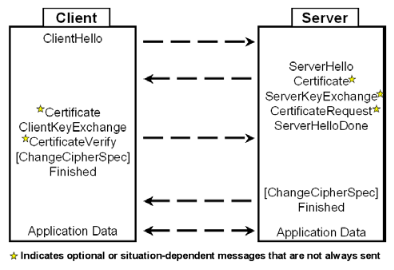
\includegraphics[width=\linewidth]{figures/handshake.png}
  \caption{Message flow for a TLS Handshake\cite{TLSHandshake}}
  \label{fig:handshake}
\end{figure}
A TLS Handshake is a exchange of multiple separate messages between server and client like seen in \Cref{fig:handshake}. As an example two of the messages are shown here:\\
The first message named ClientHello from the client to the server consists of:
\begin{itemize}
    \item The highest supported TLS Version
    \item The current time as a unix timestamp
    \item Randomly generated 28 bytes
    \item A list of Cipher suites supported by the Client
    \item A list of Compression algorithms supported by the Client
    \item A Session ID if the Client wants to resume an old Session.
    \item A list of TLS extensions
\end{itemize}
The first response from the server to the client named ServerHello consists of:
\begin{itemize}
    \item The TLS version to use
    \item Another randomly generated 28 bytes
    \item The new Session ID
    \item The cipher suite to use
    \item The compression method to use
    \item A list of TLS extensions
\end{itemize}
An example for a TLS extension is X.509\cite{rfc7633}, the extension used for certificates.

\subsection{Record}
The Record Protocol is using the information provided by the Handshake Protocol, in other words the cipher suite, the shared secret and the random values generated by both parties, to initialize the parameters for further encryption. The further encryption depends on the selected cipher suite. An encrypted message is always sent together with the MAC of the message to ensure authenticity and integrity after the handshake.\cite{rfc5246}

\subsection{Security}
Considering the lifetime of TLS, the publicized security flaws are mostly either insecure cipher suites, which can somewhat easily get removed from active use or errors in the implementation, implementation issues or other issues not related to TLS itself like stealing private keys.\cite{rfc7457}

Also of note is that if TLS is used without the usage of proper checking of certificates or public keys, a Man-in-the-Middle attack is possible. For example SSH with just a password, without certificate can be exploited.


% =============== TLS 1.2 -> TLS 1.3 ===============
\section{Transition TLS 1.2 $\rightarrow$ 1.3}

% https://datatracker.ietf.org/doc/rfc8446/?include_text=1 --- 1.2.  Major Differences from TLS 
% for each
% \subsection{Removal of legacy algorithms}
Like in every revision of the TLS standard old cipher suites have been deprecated. This time a lot more has changed though\cite{rfc8446}.

\subsection{Removal of static RSA and Diffie-Hellman cipher suites}
Forward secrecy is a feature which enhances the security of past sessions when the private key of the server or a different session key gets compromised. After all cipher suites with static RSA and Diffie-Hellman key exchange got removed, every remaining cipher suite now provides forward secrecy.
\subsection{Encryption of most handshake messages}
Because of the redesign of the handshake, every message after the ServerHello Message is encrypted, so even the certificate check is already encrypted. This adds additional privacy.
\subsection{Key derivation function redesign}
The new key derivation function is now more complex with usage of a HMAC-based Extract-and-Expand Key Derivation Function\cite{rfc5869} with the secret as an input with the addition of the handshake transcript, which includes the initial ClientHello message and as such Randomness.
\subsection{Redesign of the handshake}
The whole handshake state machine has been reworked and such many messages are now unnecessary and have been removed where possible. This reduces maintainability issues in the implementation and makes the internal structure more coherent. Also in general the default round trip time has been reduced from 3-RTT to 1-RTT, which roughly doubles the speed of the handshake.\\
The security of the handshake is mostly unchanged and is still proven to work reliably and securely\cite{7546519}.
\subsection{New Cipher suites introduced into base spec}
Cipher suites containing elliptic curve algorithms are now introduced, promising speed increases and key size decrease.
\subsection{Various other cryptographic improvements}
One of the features that has produced a few security risks was compression. This now got removed, as it wasn't useful in many use cases anyways. Other small features got changes also.
\subsection{Session resumption redesign}
Session resumption has changed dramatically in TLS 1.3 anyways and such has been replaced by an entirely new system to simplify the resumption of prior sessions.
\subsection{0-RTT}
In TLS 1.3 0 round trip time is implemented. The server dispatches the first data package in his first response and such the handshake is sped up in some special cases. 
% =============== 0-RTT ===============
\section{0-RTT}
\begin{figure}
  \includesvg[width=\linewidth]{figures/0rtt.svg}
  \caption{0-RTT handshake}
\end{figure}
Even in the new improved handshake TLS 1.3 still needs to make a whole exchange before actually sending the first packages or actual data, so TLS 1.3 introduced a system which allows the client to send data in the first round trip.\\
\subsection{Reason}
Every time the other partner needs to wait for the other party to respond, time is wasted where one of the parties needs to wait unnecessarily. With current internet connections this time might only be a few hundred milliseconds, but in high performance applications or situations where connection speed is limited, like mobile internet, it quickly adds up. For example if the internet connection has a latency of 1000 milliseconds, a TLS 1.2 handshake can take multiple seconds, where as a 0-RTT request might get answered in only one second.\\
Every round trip also includes unnecessary data needed for the messages, like for example TCP headers, so reduction of round trips also improves the bandwith used for the handshake.
\subsection{Implementation}
Encryption always needs keys and in the case of 0-RTT a secret from the last connection is used.
In TLS the shared secret can either be obtained externally or is reused from the last connection\cite{rfc8446}.
In general TLS uses the last session key, or a hashed version of the last session.
\subsection{Risks}
Because the Server has no interaction with the sent encrypted message, the security naturally degrades.
\subsubsection{Forward Secrecy}
One obvious flaw is that forward security is not provided because the message is encrypted with the last session key and if that is compromised, the attacker can also decrypt this single message. This does not compromise further communication as this key is only used once.
It is thought of a performance optimizing extension and should be enabled only by experienced users.
\subsubsection{Replay Attack}
Another flaw is the possibility of a Replay attack where an attacker can force the server to process a 0-RTT encrypted message twice\cite{7961952}. The attacker can not read or modify the message, but if 0-RTT is used incorrectly, a potential situation is, that a money transaction in online banking would be executed twice. This is not protected against in 1.3, but can instead be fought via a few different possible techniques like removing each session key after it gets used, but most of them are unfeasible at larger scale as the performance impact of those solution is rather high\cite{rfc8446}.
Due to these reasons it is recommended to only enable 0-RTT on sites it is safe to send messages multiple times, like static pages where the answer is static and no authentication in the application layer is done, as credentials could be leaked otherwise\cite{rfc8446}.

% =============== QUIC ===============
\section{QUIC}
QUIC is a network protocol which is intended to replace TCP in various applications\cite{ietf-quic-transport-16}. In particular we will have look at how QUIC uses TLS as its security layer.\cite{ietf-quic-tls-16}.

\subsection{QUIC technology explained}
Currently QUIC has a proposed standard which the latest draft is from the 23rd of October 2018\cite{ietf-quic-transport-16} with the additional 1.3 over QUIC\cite{ietf-quic-tls-16}, but is not finalized yet and is such subject to change.\\
QUIC is using UDP to reduce unnecessary round trips and delays when using TCP and at the same time embedding TLS 1.3 security into the connection for establishing quick TLS connections.\\
TCP is great if bandwith and latency isn't directly a problem, but in the current age, as page loading speed go into the range of milliseconds, the initial handshake is taking more and more time in comparison to the actual data exchange and TCP itself bloats the connection time. Package loss and other connection issues handled by TCP are becoming less and less of a problem as hardware improves. Therefore a transport layer based on UDP can reach much faster connection times without much detriment as long as a few simple checks are implemented.
Another hurdle of not using TCP is that packages typically not arrive in order with UDP based protocols or not arrive at all. TLS requires a transport protocol to reliably transport packages, so TLS itself needs to be changed quite a bit to account for the potential reordering of packages.\\
QUIC is now regarded as safe, but compromised have been made to get to the increased speed.\cite{7163028} 
\subsection{How does TLS work with QUIC?}
One of the big changes QUIC does to make TLS fit into its system is not using TLS record protection, but instead it uses it's own CRYPTO Frames. Any typical handshake packages are assigned a encryption level. For example 0 when we first send data to the server and we already had a connection before and are trying to use 0-RTT. Additionally multiple 0-RTT packages can be sent. The server then answers with the usual Handshake message with a higher encryption level. After the client receives this package, every further package is then using the new session key and after the first encrypted package arrives at the server, no Package with the 0-RTT encryption level gets accepted anymore.
\subsection{Does it do anything better?}
\begin{figure}
  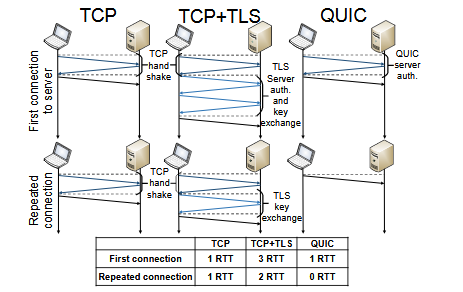
\includegraphics[width=\linewidth]{figures/rttspeed.png}
  \caption{Round Trips in TCP alone, TCP+TLS and QUIC+TLS\cite{7510788}}
  \label{fig:rtt}
\end{figure}
QUIC is being pushed by the industry for enhancing the speed of various applications and in theory the handshake is requiring less round trips in any case as seen in \cref{fig:rtt}, although is has been shown that QUIC is subpar to TCP when large amounts of data are transmitted. In most cases QUIC is faster than TCP though\cite{7510788}.
 In terms of the 0-RTT replay attack though, for QUIC it is also recommended to only enable 0-RTT for non-idempotent actions just like in TLS 1.3 alone\cite{ietf-quic-tls-16}.


% =============== CONCLUSION ===============
\section{Conclusion}
In conclusion TLS is an important technology for securing almost everything in the current internet and is doing a good job at it, but it has inherited a lot of legacy technology and it is slowly getting rid of all substandard ciphers and design flaws. TLS 1.3 is a step into a faster and more secure internet by further removing deprecated algorithms and reworking old designs.\\
0-RTT and 1-RTT is a huge step for a faster internet as less time is wasted in doing handshakes and a more responsive internet without adding better hardware is always a goal to strive for. Additionally forward secrecy is another way to keep information secure in the future.
QUIC is potentially another big step into an even faster internet by trying to switch out a de facto standard since the internet started. Since most of the cryptographic background is coming from TLS 1.3 and such is secure, QUIC seems to be a great improvement if it gets widespread implementation.
% =============== REFERENCES ===============
\bibliography{references}

\end{document}